\section{Background}
\label{game:background}
%Pontsification - not enough
Gamification is not about taking an already existing system and decorating it with points, levels and leaderboards. This methodology of gamifying a system is referred to as "Pontsification" where the game design exclusively relies on points, badges and leaderboards \cite{47}. Zichermann et al \cite{48} argues that the technique of "Pointsification" comes as a result of lacking creativity and represents a poor approach to gamification. In order to create a gamified system that truly engages users and affects their needs for satisfaction, a game designer should put more work and effort than just throwing points, badges and leaderboards into the system hoping for users to feel engaged. 

The \ac{sdt} and its sub-theory \ac{cet} have been explained in Section \ref{thb:gamedesign} and serve as the foundations on which we base our gamification model and aim to reach the goal of positively affecting users needs for satisfaction, which (accrding to \ac{sdt} and \ac{cet}) results in increased intrinsic motivation. Before we proceed with state-of-the-art gameified systems, it is important to understand some key concepts that compose a well designed game. In gamification, the most frequently used framework is the MDA Framework \cite{47}. It is one of the most leveraged frameworks of game design and it is an abbreviation of the terms: Mechanics, Dynamics and Aesthetics.
% MDA framework
\begin{itemize}
    \item \textbf{Mechanics} compose the functioning of the game. Mechanics allow a designer to have complete control over the levels of the game, giving the ability to guide the players' actions
    \item \textbf{Dynamics} are the interactions of a player with the game mechanics. They determine the action of the player in response to the mechanics of the system
    \item \textbf{Aesthetics} of the game are the elements that define how the player is feeling during his/her interaction with the game
\end{itemize}
 
By carefully studying and exploring these models and frameworks when working on the game design, it will be genuinely possible to transform a system from being monotone and tedious to something that is interactive and fun to do. 

% Stats on game play 
A well designed game or gamified system can be used to gather large-scale amount of data and information. This data can potentially open doors to improving advanced systems such as search engines or helping scientific researchers find solutions to complex protein structures by using the computing power of the people (See Foldit \cite{53}). Entertainment Software Association did a survey to find out what are the characteristics of an average gamer and how much time gamers spent playing video games, and the following statistics were reported \cite{49}:
\begin{itemize}
    \item An approximation of 5 million Americans will spend 40 or more hours a week playing games, which is the equivalent of a full time job
    \item 60\% of Americans are gamers
    \item During 2013 the gaming industry was worth 22 billion dollars, with 16 billion spent on game content only 
    \item Females account for 50\% of gameplay and purchases
    \item The average gamer is 36 years old
\end{itemize}


\newpage
\begin{figure}[]
  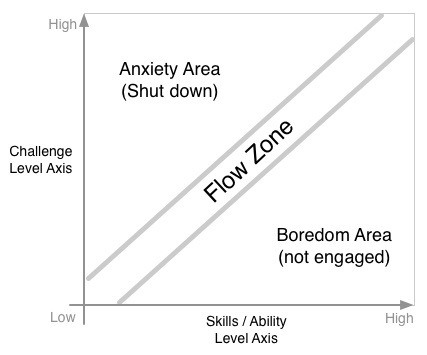
\includegraphics[width=.8\linewidth]{figures/experiment2/flowzone.png}
  \caption{The flow zone of a gameplay \cite{49}}
  \label{fig:flowzone}
\end{figure}
%Flow zone
A very important aspect in game design is the ability of maintaining the so called "Flow Zone" during the gameplay. The success of a game is achieved if the player is constantly kept within the flow-zone which is placed between anxiety and boredom \cite{49}. As illustrated in Figure \ref{fig:flowzone}, achieving flow or being in the "flow-zone" indicates the players' state of not being too overwhelmed with challenges but also avoiding the state of being bored because the game continues to offer easy challenges to the player. Zichermann et al. \cite{48} argues that a game designer must create a careful interplay of the system with the player by relentlessly testing their interactions until the point in which the player is between anxiety and boredom. This rule is applied from the first interaction of the player with the system which brings us to another quite important point in game design: Onboarding. 

%importance of onboarding 
According to Zichermann et al. \cite{48}, statistics from the casual games market show that the first minutes a player interacts with the game are the most important. This is because during the first minutes the player makes a decision whether he/she likes the game and will continue to play or not. Therefore, onboarding plays a crucial role to the overall success of the game. Onboarding is defined by Zichermann as the act of bringing novice players into the system. The responsibility of this part of the game is to carefully reveal the complexity of the system to the player without overwhelming him with too much information. In short, the goal of onboarding is to train and engage players but not overwhelm them.

%importance of challegne and other aspects (the bulletlist on the last th.b. page in the notebook about gamification).
Finally, some aspects which contribute to the idea of keeping the player engaged and motivated during gameplay need to be pointed out before we proceed with the next sections. According to Siemens et al. \cite{49}, a player expects the following elements from the game:
\begin{itemize}
    \item Focused goals
    \item Challenging tasks
    \item Clear and compelling standards
    \item Protection from failure
    \item Affirmation
    \item Novelty
    \item Freedom of choice
    \item Authenticity
    \item Affiliation with others
\end{itemize}
For our Fastype Game we have tried to employ most of these important aspects of game design in order to achieve high levels of engagement and intrinsically motivate players to interact with the game without any other form of incentive except the incentive of being entertained.